% Unofficial University of Cambridge Poster Template
% https://github.com/andiac/gemini-cam
% a fork of https://github.com/anishathalye/gemini
% also refer to https://github.com/k4rtik/uchicago-poster

\documentclass[final]{beamer}

% ====================
% Packages
% ====================

\usepackage[T1]{fontenc}
\usepackage{lmodern}
\usepackage[orientation=portrait,size=custom,width=120,height=120,scale=1]{beamerposter}
\usetheme{gemini}
\usepackage[dvipsnames]{xcolor}
\usecolortheme{nott}
\usepackage{graphicx}
\usepackage{booktabs}
\usepackage{tikz}
\usetikzlibrary{patterns,decorations.pathmorphing}
\usepackage{tkz-euclide}
\tikzset{point style/.style = {%
  draw = black,
  inner sep = 0pt,
  shape = circle,
  minimum size = 5pt,
  fill = black
 },
 every picture/.append style = {
  scale = 1.5
 },
 every node/.append style={
  scale=1.5
 }
}
\usepackage{pgfplots}
\pgfplotsset{compat=1.14}
\usepackage{anyfontsize}
\usepackage{caption}
\usepackage{subcaption}

% ====================
% Lengths
% ====================

% If you have N columns, choose \sepwidth and \colwidth such that
% (N+1)*\sepwidth + N*\colwidth = \paperwidth
\newlength{\sepwidth}
\newlength{\colwidth}
\setlength{\sepwidth}{0.01\paperwidth}
\setlength{\colwidth}{0.32\paperwidth}

\newcommand{\separatorcolumn}{\begin{column}{\sepwidth}\end{column}}
\newcommand{\bfalert}[1]{\textbf{\alert{#1}}}

% Math shortcuts
\newcommand{\R}{\mathbb{R}}

% ====================
% Title
% ====================

\title{Polygons \& Transformations Cheatsheet}

\author{3.AB PreIB Math}

\institute[shortinst]{Adam Klepáč}

% ====================
% Footer (optional)
% ====================

% \footercontent{
%   \href{https://utfpr.edu.br/ct/ppgca}{utfpr.edu.br/ct/ppgca} \hfill
%   Mostra de Trabalhos do PPGCA --- TechTalks 2024 \hfill
%   \href{mailto:ppgca-ct@utfpr.edu.br}{ppgca-ct@utfpr.edu.br}}
% (can be left out to remove footer)


% ====================
% Logo (optional)
% ====================

% use this to include logos on the left and/or right side of the header:
\logoright{
\includegraphics[height=3.5cm]{logos/logo-white.png}}
% \logoleft{\hspace{20ex}\includegraphics[height=3.5cm]{logos/ppgca-logo.png}}

% ====================
% Body
% ====================

\begin{document}

% Refer to https://github.com/k4rtik/uchicago-poster
% logo: https://www.cam.ac.uk/brand-resources/about-the-logo/logo-downloads
% \addtobeamertemplate{headline}{}
% {
%     \begin{tikzpicture}[remember picture,overlay]
%       \node [anchor=north west, inner sep=3cm] at ([xshift=-2.5cm,yshift=1.75cm]current page.north west)
%       {\includegraphics[height=7cm]{logos/unott-logo.eps}}; 
%     \end{tikzpicture}
% }

\begin{frame}[t]
\begin{columns}[t]
\separatorcolumn

\begin{column}{\colwidth}

  \begin{block}{Polygons}

   Polygon is a \bfalert{closed} 2D shape \bfalert{made only of segments}. We
   call the endpoints of those segments, \bfalert{vertices}, and the segments
   themselves, \bfalert{edges}.

   \textbf{Examples}
   \begin{figure}[H]
    \centering
    \begin{subfigure}[b]{.23\textwidth}
     \centering
     \begin{tikzpicture}
      \tkzDefPoint(0:1){A}
      \tkzDefPoint(110:2){B}
      \tkzDefPoint(180:1){C}

      \tkzDrawPoints(A,B,C);
      \tkzDrawSegments[thick](A,B B,C C,A);
     \end{tikzpicture}
     \caption*{Triangle}
    \end{subfigure}
    \begin{subfigure}[b]{.23\textwidth}
     \centering
     \begin{tikzpicture}
      \tkzDefPoint(0:1){A}
      \tkzDefPoint(60:1.5){B}
      \tkzDefPoint(130:2.5){C}
      \tkzDefPoint(180:1){D}

      \tkzDrawPoints(A,B,C,D);
      \tkzDrawSegments[thick](A,B B,C C,D D,A);
     \end{tikzpicture}
     \caption*{Quadrilateral}
    \end{subfigure}
    \begin{subfigure}[b]{.23\textwidth}
     \centering
     \begin{tikzpicture}
      \tkzDefPoint(0:1){A}
      \tkzDefPoint(50:2){B}
      \tkzDefPoint(90:2){C}
      \tkzDefPoint(120:2){D}
      \tkzDefPoint(180:1){E}

      \tkzDrawPoints(A,B,C,D,E);
      \tkzDrawSegments[thick](A,B B,C C,D D,E E,A);
     \end{tikzpicture}
     \caption*{Pentagon}
    \end{subfigure}
    \begin{subfigure}[b]{.27\textwidth}
     \centering
     \begin{tikzpicture}
      \tkzDefPoint(0:1){A}
      \tkzDefPoint(13:2){B}
      \tkzDefPoint(30:2.5){C}
      \tkzDefPoint(50:2){D}
      \tkzDefPoint(70:1){E}
      \tkzDefPoint(86:2){F}
      \tkzDefPoint(97:1.5){G}
      \tkzDefPoint(109:2){H}
      \tkzDefPoint(121:2){I}
      \tkzDefPoint(140:1.5){J}
      \tkzDefPoint(160:1){K}
      \tkzDefPoint(180:1){L}

      \tkzDrawPoints(A,B,C,D,E,F,G,H,I,J,K,L);
      \tkzDrawSegments[thick](A,B B,C C,D D,E E,F F,G G,H H,I I,J J,K K,L L,A);
     \end{tikzpicture}
     \caption*{Dodecagon}
    \end{subfigure}
   \end{figure}
   Polygons with $n$ sides are called \bfalert{$n$-gons}.

   \textbf{Counterexamples}
   \begin{figure}[H]
    \centering
    \begin{subfigure}[b]{.32\textwidth}
     \centering
     \begin{tikzpicture}
      \tkzDefPoint(0:1){A}
      \tkzDefPoint(90:1){B}
      \tkzDefPoint(150:1){C}

      \tkzDrawPoints(A,B,C);
      \tkzDrawSegments[thick](A,B B,C);
     \end{tikzpicture}
     \caption*{Not closed}
    \end{subfigure}
    \begin{subfigure}[b]{.32\textwidth}
     \centering
     \begin{tikzpicture}[scale=2]
      \tkzDefPoint(0,0){A1}
      \tkzDefPoint(0,1){B1}
      \tkzDefPoint(1,1){C1}
      \tkzDefPoint(1,0){D1}

      \tkzDefPoint(0.5,0.3){A2}
      \tkzDefPoint(0.5,1.3){B2}
      \tkzDefPoint(1.5,1.3){C2}
      \tkzDefPoint(1.5,0.3){D2}
      \tkzDrawPoints(A1,B1,C1,D1,A2,B2,C2,D2)

      \tkzDrawSegments[thick](A1,B1 B1,C1 C1,D1 D1,A1 B2,C2 C2,D2 B1,B2 C1,C2 D1,D2)
      \tkzDrawSegments[dashed,thick](A2,B2 D2,A2 A1,A2)
     \end{tikzpicture}
     \caption*{3D}
    \end{subfigure}
    \begin{subfigure}[b]{.32\textwidth}
     \centering
     \begin{tikzpicture}
      \tkzDefPoint(0:1){A}
      \tkzDefPoint(180:1){B}
      \tkzDefPoint(90:1){P}

      \tkzDrawPoints(A,B)
      \tkzDrawArc[thick](P,A)(B)
      \tkzDrawSegment[thick](A,B)
     \end{tikzpicture}
     \caption*{Not straight}
    \end{subfigure}
   \end{figure}
  \end{block}

  \begin{block}{Convex Polygons}

   A polygon is called \bfalert{convex} if it has no internal angle greater than
   180$^{\circ}$.
   \begin{figure}[H]
    \centering
    \begin{subfigure}[b]{.35\textwidth}
     \centering
     \begin{tikzpicture}[scale=1.5]
      \tkzDefPoint(0:1){A}
      \tkzDefPoint(50:2){B}
      \tkzDefPoint(90:2){C}
      \tkzDefPoint(120:2){D}
      \tkzDefPoint(180:1){E}

      \tkzDrawPoints[color=gevoblue](A,B,C,D,E);
      \tkzDrawSegments[color=gevoblue,thick](A,B B,C C,D D,E E,A);
     \end{tikzpicture}
     \caption*{\textcolor{gevoblue}{Convex}}
    \end{subfigure}
    \begin{subfigure}[b]{.35\textwidth}
     \centering
     \begin{tikzpicture}[scale=1.5]
      \tkzDefPoint(0,0){A}
      \tkzDefPoint(2,0){B}
      \tkzDefPoint(2,2){C}
      \tkzDefPoint(1,1){D}
      \tkzDefPoint(0,2){E}

      \tkzDrawPoints[color=gevored](A,B,C,D,E)
      \tkzDrawSegments[color=gevored,thick](A,B B,C C,D D,E E,A)

      \tkzMarkAngle[color=gevored,size=0.65,thick](E,D,C)
      \tkzLabelAngle[color=gevored,pos=0.25](E,D,C){\footnotesize $>\!\!180^{\circ}$}
     \end{tikzpicture}
     \caption*{\textcolor{gevored}{NOT convex}}
    \end{subfigure}
   \end{figure}

   \textbf{Special types of convex polygons}
   \begin{figure}[H]
    \centering
    \begin{subfigure}[b]{.3\textwidth}
     \begin{tikzpicture}[scale=2]
      \tkzDefPoint(0,0){A}
      \tkzDefPoint(0.3,1){B}
      \tkzDefPoint(1,1){C}
      \tkzDefPoint(2,0){D}

      \tkzDrawPolygon[thick](A,B,C,D)
      \tkzDrawSegments[ultra thick,gevodarkblue](B,C A,D)
      \tkzDrawPoints(A,B,C,D)
     \end{tikzpicture}
     \caption*{\alert{Trapezoid/Trapezium}\\ 
      A convex quadrilateral with at least two parallel sides.}
    \end{subfigure}
    \begin{subfigure}[b]{.3\textwidth}
     \begin{tikzpicture}[scale=2]
      \tkzDefPoint(0,0){A}
      \tkzDefPoint(0.5,0.75){B}
      \tkzDefPoint(2,0.75){C}
      \tkzDefPoint(1.5,0){D}

      \tkzDrawSegments[ultra thick,gevodarkblue](B,C A,D)
      \tkzDrawSegments[ultra thick,gevodarkred](A,B C,D)
      \tkzDrawPoints(A,B,C,D)
     \end{tikzpicture}
     \caption*{\alert{Parallelogram}\\
      A convex quadrilateral with two pairs of parallel sides.}
    \end{subfigure}
    \begin{subfigure}[b]{.3\textwidth}
     \begin{tikzpicture}[scale=2]
      \clip (-0.04,-0.04) rectangle (1.44,0.79);
      \tkzDefPoint(0,0){A}
      \tkzDefPoint(0.5,0.75){B}
      \tkzDefPoint(1.4,0.75){C}
      \tkzDefPoint(0.9,0){D}

      \tkzDrawPolygon[ultra thick,gevodarkblue](A,B,C,D)
      \tkzDrawPoints(A,B,C,D)
      \tkzDrawSegments[thick](A,C B,D)
      \tkzInterLL(A,C)(B,D) \tkzGetPoint{O}
      \tkzMarkAngle[size=0.2](A,O,D)
      \tkzLabelAngle[pos=0.1](A,O,D){$ \cdot $}
     \end{tikzpicture}
     \caption*{\alert{Rhombus}\\
     An \textbf{equilateral} (all sides of the same length) parallelogram.}
    \end{subfigure}
   \end{figure}

   In addition, if a \textbf{convex} polygon has \textbf{all sides of the same
   length} and \textbf{all angles of the same size}, it is called
   \bfalert{regular}.
   \begin{figure}[H]
    \captionsetup{justification=centering}
    \centering
    \begin{subfigure}[t]{.24\textwidth}
     \centering
     \begin{tikzpicture}
      \tkzDefPoint(-30:1){A}
      \tkzDefPoint(90:1){B}
      \tkzDefPoint(210:1){C}
       
      \tkzDrawPolygon[thick](A,B,C)
      \tkzDrawPoints(A,B,C)
     \end{tikzpicture}
     \caption*{Equilateral triangle (regular trigon)}
    \end{subfigure}
    \begin{subfigure}[t]{.24\textwidth}
     \centering
     \begin{tikzpicture}
      \tkzDefPoint(-45:1){A}
      \tkzDefPoint(-135:1){B}
      \tkzDefPoint(135:1){C}
      \tkzDefPoint(45:1){D}
       
      \tkzDrawPolygon[thick](A,B,C,D)
      \tkzDrawPoints(A,B,C,D)
     \end{tikzpicture}
     \caption*{Square (regular tetragon)}
    \end{subfigure}
    \begin{subfigure}[t]{.24\textwidth}
     \centering
     \begin{tikzpicture}
      \tkzDefPoint(-54:1){A}
      \tkzDefPoint(18:1){B}
      \tkzDefPoint(90:1){C}
      \tkzDefPoint(162:1){D}
      \tkzDefPoint(234:1){E}
       
      \tkzDrawPolygon[thick](A,B,C,D,E)
      \tkzDrawPoints(A,B,C,D,E)
     \end{tikzpicture}
     \caption*{Regular pentagon}
    \end{subfigure}
    \begin{subfigure}[t]{.24\textwidth}
     \centering
     \begin{tikzpicture}
      \tkzDefPoint(0:1){A}
      \tkzDefPoint(60:1){B}
      \tkzDefPoint(120:1){C}
      \tkzDefPoint(180:1){D}
      \tkzDefPoint(240:1){E}
      \tkzDefPoint(300:1){F}
       
      \tkzDrawPolygon[thick](A,B,C,D,E,F)
      \tkzDrawPoints(A,B,C,D,E,F)
     \end{tikzpicture}
     \caption*{Regular hexagon}
    \end{subfigure}
   \end{figure}
  \end{block}

  \begin{exampleblock}{Diagonals \& Triangulations}

   A \bfalert{diagonal} in a \textbf{convex} polygon is a segment connecting two
   of its \textbf{non-adjacent} vertices.
   \begin{figure}[H]
    \centering
    \begin{tikzpicture}
     \tkzDefPoint(0,0){A}
     \tkzDefPoint(-1,0.5){B}
     \tkzDefPoint(0.3,2){C}
     \tkzDefPoint(2,1){D}
     \tkzDefPoint(2,0.5){E}
     \tkzDefPoint(1.5,0){F}
     \tkzDrawPolygon(A,B,C,D,E,F)
     \tkzDrawSegment[color=gevored,ultra thick](A,D)
     \tkzDrawPoints(A,B,C,D,E,F)
    \end{tikzpicture}
    \caption*{\textcolor{gevored}{Diagonal} in a convex hexagon.}
   \end{figure}

   A \bfalert{triangulation} of a \textbf{convex} polygon is its division into
   triangles by \textbf{non-intersecting} diagonals.

   \begin{figure}[H]
    \centering
    \begin{subfigure}[b]{.2\textwidth}
     \centering
     \begin{tikzpicture}[scale=0.875]
      \tkzDefPoint(-45:1){A}
      \tkzDefPoint(-135:1){B}
      \tkzDefPoint(135:1){C}
      \tkzDefPoint(45:1){D}

      \tkzDrawPolygon(A,B,C,D)
      \tkzDrawSegment[ultra thick,gevored](A,C)
      \tkzDrawPoints(A,B,C,D)
     \end{tikzpicture}
    \end{subfigure}
    \begin{subfigure}[b]{.2\textwidth}
     \centering
     \begin{tikzpicture}[scale=0.7]
      \tkzDefPoint(0:1){A}
      \tkzDefPoint(60:1){B}
      \tkzDefPoint(120:1){C}
      \tkzDefPoint(180:1){D}
      \tkzDefPoint(240:1){E}
      \tkzDefPoint(300:1){F}

      \tkzDrawPolygon(A,B,C,D,E,F)
      \tkzDrawSegments[ultra thick,color=gevored](A,C D,F A,D)
      \tkzDrawPoints(A,B,C,D,E,F)
     \end{tikzpicture}
    \end{subfigure}
    \begin{subfigure}[b]{.2\textwidth}
     \centering
     \begin{tikzpicture}[scale=0.7]
      \tkzDefPoint(0:1){A}
      \tkzDefPoint(60:1){B}
      \tkzDefPoint(120:1){C}
      \tkzDefPoint(180:1){D}
      \tkzDefPoint(240:1){E}
      \tkzDefPoint(300:1){F}

      \tkzDrawPolygon(A,B,C,D,E,F)
      \tkzDrawSegments[ultra thick,color=gevored](B,D D,F B,F)
      \tkzDrawPoints(A,B,C,D,E,F)
     \end{tikzpicture}
    \end{subfigure}
    \caption*{Examples of \textcolor{gevored}{triangulations}.}
   \end{figure}

   \begin{figure}[H]
    \centering
    \begin{subfigure}[b]{.2\textwidth}
     \centering
     \begin{tikzpicture}[scale=0.875]
      \tkzDefPoint(-45:1){A}
      \tkzDefPoint(-135:1){B}
      \tkzDefPoint(135:1){C}
      \tkzDefPoint(45:1){D}

      \tkzDrawPolygon(A,B,C,D)
      \tkzDrawSegments[ultra thick,gevored](A,C B,D)
      \tkzDrawPoints(A,B,C,D)
     \end{tikzpicture}
    \end{subfigure}
    \begin{subfigure}[b]{.2\textwidth}
     \centering
     \begin{tikzpicture}[scale=0.7]
      \tkzDefPoint(0:1){A}
      \tkzDefPoint(60:1){B}
      \tkzDefPoint(120:1){C}
      \tkzDefPoint(180:1){D}
      \tkzDefPoint(240:1){E}
      \tkzDefPoint(300:1){F}

      \tkzDrawPolygon(A,B,C,D,E,F)
      \tkzDrawSegments[ultra thick,color=gevored](A,C A,E)
      \tkzDrawPoints(A,B,C,D,E,F)
     \end{tikzpicture}
    \end{subfigure}
    \begin{subfigure}[b]{.2\textwidth}
     \centering
     \begin{tikzpicture}[scale=0.7]
      \tkzDefPoint(0:1){A}
      \tkzDefPoint(60:1){B}
      \tkzDefPoint(120:1){C}
      \tkzDefPoint(180:1){D}
      \tkzDefPoint(240:1){E}
      \tkzDefPoint(300:1){F}

      \tkzDrawPolygon(A,B,C,D,E,F)
      \tkzDrawSegments[ultra thick,color=gevored](B,E C,F B,F)
      \tkzDrawPoints(A,B,C,D,E,F)
     \end{tikzpicture}
    \end{subfigure}
    \caption*{Counterexamples of \textcolor{gevored}{triangulations}.}
   \end{figure}

   The total number of different triangulations of a convex $n$-gon is
   \[
    \frac{n \cdot (n+1) \cdot \ldots \cdot (2n - 4)}{(n-2)!},
   \]
   which you \textbf{of course don't have to remember}. Interestingly enough,
   every triangulation can be transformed into any other by a series of
   \bfalert{flips}.

   A \bfalert{flip} is a swap of one diagonal for the other in a chosen
   quadrilateral so that the \textbf{result is again a triangulation}.
   \begin{figure}[H]
    \centering
    \begin{subfigure}[b]{.4\textwidth}
     \centering
     \begin{tikzpicture}[scale=0.7]
      \begin{scope}
       \tkzDefPoint(0:1){A}
       \tkzDefPoint(60:1){B}
       \tkzDefPoint(120:1){C}
       \tkzDefPoint(180:1){D}
       \tkzDefPoint(240:1){E}
       \tkzDefPoint(300:1){F}

       \tkzDrawPolygon(A,B,C,D,E,F)
       \tkzDrawPolygon[fill,pattern={north west lines},pattern
       color=black!50](B,D,E,F)
       \tkzDrawSegments[ultra thick,color=gevored](B,D B,F)
       \tkzDrawSegment[ultra thick,color=gevodarkblue](D,F)
       \tkzDrawPoints(A,B,C,D,E,F)
      \end{scope}
      \begin{scope}[xshift=2cm]
       \draw[ultra thick,gevodarkblue,->] (0,0) -- (2,0);
      \end{scope}
      \begin{scope}[xshift=6cm]
       \tkzDefPoint(0:1){A}
       \tkzDefPoint(60:1){B}
       \tkzDefPoint(120:1){C}
       \tkzDefPoint(180:1){D}
       \tkzDefPoint(240:1){E}
       \tkzDefPoint(300:1){F}

       \tkzDrawPolygon(A,B,C,D,E,F)
       \tkzDrawPolygon[fill,pattern={north west lines},pattern
       color=black!50](B,D,E,F)
       \tkzDrawSegments[ultra thick,color=gevored](B,D B,F)
       \tkzDrawSegment[ultra thick,color=gevodarkblue](B,E)
       \tkzDrawPoints(A,B,C,D,E,F)
      \end{scope}
     \end{tikzpicture}
    \end{subfigure}
    \begin{subfigure}[b]{.4\textwidth}
     \centering
     \begin{tikzpicture}[scale=0.7]
      \begin{scope}[rotate=18]
       \tkzDefPoint(0:1){A}
       \tkzDefPoint(72:1){B}
       \tkzDefPoint(144:1){C}
       \tkzDefPoint(216:1){D}
       \tkzDefPoint(288:1){E}

       \tkzDrawPolygon(A,B,C,D,E)
       \tkzDrawPolygon[fill,pattern={north west lines},pattern
       color=black!50](A,C,D,E)
       \tkzDrawSegment[ultra thick,color=gevored](A,C)
       \tkzDrawSegment[ultra thick,color=gevodarkblue](A,D)
       \tkzDrawPoints(A,B,C,D,E)
      \end{scope}
      \begin{scope}[xshift=2cm]
       \draw[ultra thick,gevodarkblue,->] (0,0) -- (2,0);
      \end{scope}
      \begin{scope}[xshift=6cm,rotate=18]
       \tkzDefPoint(0:1){A}
       \tkzDefPoint(72:1){B}
       \tkzDefPoint(144:1){C}
       \tkzDefPoint(216:1){D}
       \tkzDefPoint(288:1){E}

       \tkzDrawPolygon(A,B,C,D,E)
       \tkzDrawPolygon[fill,pattern={north west lines},pattern
       color=black!50](A,C,D,E)
       \tkzDrawSegment[ultra thick,color=gevored](A,C)
       \tkzDrawSegment[ultra thick,color=gevodarkblue](C,E)
       \tkzDrawPoints(A,B,C,D,E)
      \end{scope}
     \end{tikzpicture}
    \end{subfigure}
    \caption*{Examples of \textcolor{gevodarkblue}{flips}.}
   \end{figure}

   \begin{figure}[H]
    \centering
    \begin{subfigure}[b]{.4\textwidth}
     \centering
     \begin{tikzpicture}[scale=0.7]
      \begin{scope}
       \tkzDefPoint(0:1){A}
       \tkzDefPoint(60:1){B}
       \tkzDefPoint(120:1){C}
       \tkzDefPoint(180:1){D}
       \tkzDefPoint(240:1){E}
       \tkzDefPoint(300:1){F}

       \tkzDrawPolygon(A,B,C,D,E,F)
       \tkzDrawSegments[ultra thick,color=gevored](B,D B,F)
       \tkzDrawSegment[ultra thick,color=gevodarkblue](D,F)
       \tkzDrawPoints(A,B,C,D,E,F)
      \end{scope}
      \begin{scope}[xshift=2cm]
       \draw[ultra thick,gevodarkblue,->,decorate,decoration={zigzag}] (0,0) --
        (2,0);
       \draw[ultra thick,gevored,rotate around={45:(1,0)}] (0.5,0) -- (1.5,0);
       \draw[ultra thick,gevored,rotate around={-45:(1,0)}] (0.5,0) -- (1.5,0);
      \end{scope}
      \begin{scope}[xshift=6cm]
       \tkzDefPoint(0:1){A}
       \tkzDefPoint(60:1){B}
       \tkzDefPoint(120:1){C}
       \tkzDefPoint(180:1){D}
       \tkzDefPoint(240:1){E}
       \tkzDefPoint(300:1){F}

       \tkzDrawPolygon(A,B,C,D,E,F)
       \tkzDrawSegments[ultra thick,color=gevored](B,D B,F)
       \tkzDrawSegment[ultra thick,color=gevodarkblue](A,E)
       \tkzDrawPoints(A,B,C,D,E,F)
      \end{scope}
     \end{tikzpicture}
    \end{subfigure}
    \begin{subfigure}[b]{.4\textwidth}
     \centering
     \begin{tikzpicture}[scale=0.7]
      \begin{scope}[rotate=18]
       \tkzDefPoint(0:1){A}
       \tkzDefPoint(72:1){B}
       \tkzDefPoint(144:1){C}
       \tkzDefPoint(216:1){D}
       \tkzDefPoint(288:1){E}

       \tkzDrawPolygon(A,B,C,D,E)
       \tkzDrawSegment[ultra thick,color=gevored](A,C)
       \tkzDrawSegment[ultra thick,color=gevodarkblue](A,D)
       \tkzDrawPoints(A,B,C,D,E)
      \end{scope}
      \begin{scope}[xshift=2cm]
       \draw[ultra thick,gevodarkblue,->,decorate,decoration={zigzag}] (0,0) --
        (2,0);
       \draw[ultra thick,gevored,rotate around={45:(1,0)}] (0.5,0) -- (1.5,0);
       \draw[ultra thick,gevored,rotate around={-45:(1,0)}] (0.5,0) -- (1.5,0);
      \end{scope}
      \begin{scope}[xshift=6cm,rotate=18]
       \tkzDefPoint(0:1){A}
       \tkzDefPoint(72:1){B}
       \tkzDefPoint(144:1){C}
       \tkzDefPoint(216:1){D}
       \tkzDefPoint(288:1){E}

       \tkzDrawPolygon(A,B,C,D,E)
       \tkzDrawSegment[ultra thick,color=gevored](A,C)
       \tkzDrawSegment[ultra thick,color=gevodarkblue](B,E)
       \tkzDrawPoints(A,B,C,D,E)
      \end{scope}
     \end{tikzpicture}
    \end{subfigure}
    \caption*{Counterexamples of \textcolor{gevodarkblue}{flips}.}
   \end{figure}

   \begin{figure}[H]
    \centering
    \begin{tikzpicture}[scale=0.7]
     \begin{scope}
      \tkzDefPoint(0:1){A}
      \tkzDefPoint(60:1){B}
      \tkzDefPoint(120:1){C}
      \tkzDefPoint(180:1){D}
      \tkzDefPoint(240:1){E}
      \tkzDefPoint(300:1){F}

      \tkzDrawPolygon(A,B,C,D,E,F)
      \tkzDrawSegments[ultra thick,color=gevored](B,D B,F D,F)
      \tkzDrawPoints(A,B,C,D,E,F)
     \end{scope}
     \begin{scope}[xshift=1.5cm]
      \draw[ultra thick,gevodarkblue,->] (0,0) -- (1,0);
     \end{scope}
     \begin{scope}[xshift=4cm]
      \tkzDefPoint(0:1){A}
      \tkzDefPoint(60:1){B}
      \tkzDefPoint(120:1){C}
      \tkzDefPoint(180:1){D}
      \tkzDefPoint(240:1){E}
      \tkzDefPoint(300:1){F}

      \tkzDrawPolygon(A,B,C,D,E,F)
      \tkzDrawSegments[ultra thick,color=gevored](C,F B,F D,F)
      \tkzDrawPoints(A,B,C,D,E,F)
     \end{scope}
     \begin{scope}[xshift=5.5cm]
      \draw[ultra thick,gevodarkblue,->] (0,0) -- (1,0);
     \end{scope}
     \begin{scope}[xshift=8cm]
      \tkzDefPoint(0:1){A}
      \tkzDefPoint(60:1){B}
      \tkzDefPoint(120:1){C}
      \tkzDefPoint(180:1){D}
      \tkzDefPoint(240:1){E}
      \tkzDefPoint(300:1){F}

      \tkzDrawPolygon(A,B,C,D,E,F)
      \tkzDrawSegments[ultra thick,color=gevored](C,F B,F C,E)
      \tkzDrawPoints(A,B,C,D,E,F)
     \end{scope}
     \begin{scope}[xshift=9.5cm]
      \draw[ultra thick,gevodarkblue,->] (0,0) -- (1,0);
     \end{scope}
     \begin{scope}[xshift=12cm]
      \tkzDefPoint(0:1){A}
      \tkzDefPoint(60:1){B}
      \tkzDefPoint(120:1){C}
      \tkzDefPoint(180:1){D}
      \tkzDefPoint(240:1){E}
      \tkzDefPoint(300:1){F}

      \tkzDrawPolygon(A,B,C,D,E,F)
      \tkzDrawSegments[ultra thick,color=gevored](C,F A,C C,E)
      \tkzDrawPoints(A,B,C,D,E,F)
     \end{scope}
     \begin{scope}[xshift=13.5cm]
      \draw[ultra thick,gevodarkblue,->] (0,0) -- (1,0);
     \end{scope}
     \begin{scope}[xshift=16cm]
      \tkzDefPoint(0:1){A}
      \tkzDefPoint(60:1){B}
      \tkzDefPoint(120:1){C}
      \tkzDefPoint(180:1){D}
      \tkzDefPoint(240:1){E}
      \tkzDefPoint(300:1){F}

      \tkzDrawPolygon(A,B,C,D,E,F)
      \tkzDrawSegments[ultra thick,color=gevored](A,E A,C C,E)
      \tkzDrawPoints(A,B,C,D,E,F)
     \end{scope}
    \end{tikzpicture}
    \caption*{Passage from one triangulation to another through a series of
    \textcolor{gevodarkblue}{flips}.}
   \end{figure}
   I encourage you to think about how to determine the number of flips necessary
   to pass from one triangulation to another. Can I have made the passage above
   in fewer flips?
  \end{exampleblock}
\end{column}

\separatorcolumn

\begin{column}{\colwidth}

 \begin{block}{Plane Transformations}
  The \bfalert{plane} is basically just the set $\R^2$ of all \textbf{pairs of
  real numbers}. A pair $(x,y) \in \R^2$ is typically called a \bfalert{point}.
  Then, a plane \bfalert{transformation} is a \textbf{function} which maps
  points to points. In symbols, it's a function $\R^2 \to \R^2$.

  We can visualise what a transformation does for example by look at the image
  of a square (or an entire grid).
  \begin{figure}[H]
   \centering
   \begin{subfigure}[c]{.2\textwidth}
    \centering
    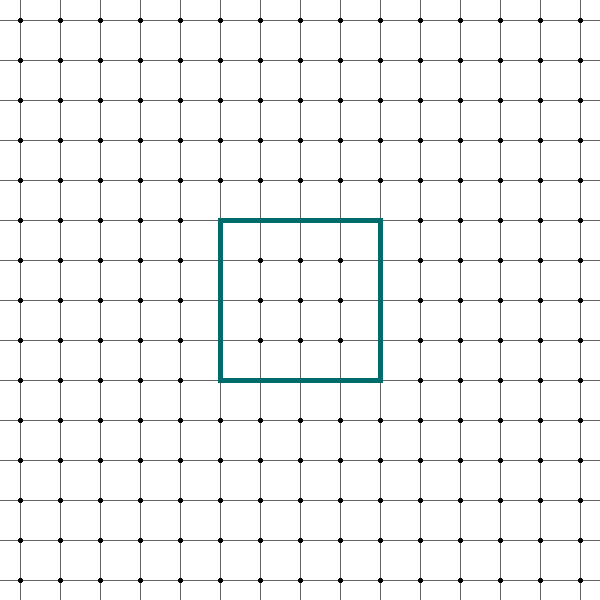
\includegraphics[width=\textwidth]{grid.png}
   \end{subfigure}
   \begin{subfigure}[c]{.1\textwidth}
    \centering
    \begin{tikzpicture}
     \draw[ultra thick,gevored,->] (0,0) -- (2,0);
    \end{tikzpicture}
   \end{subfigure}
   \begin{subfigure}[c]{.2\textwidth}
    \centering
    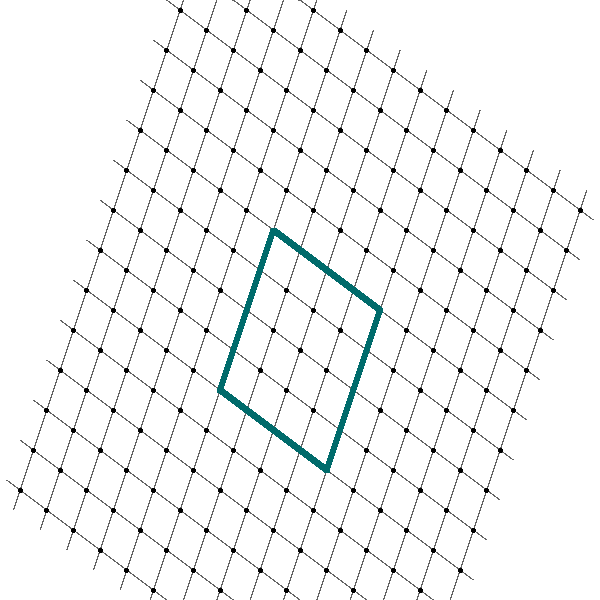
\includegraphics[width=\textwidth]{transformed_grid_2.png}
   \end{subfigure}
   \caption*{The transformation \alert{$(x,y) \mapsto (\frac{1}{3}(2x - y),
   \frac{1}{2}(x + 2y))$}.}
  \end{figure}

  \begin{figure}[H]
   \centering
   \begin{subfigure}[c]{.2\textwidth}
    \centering
    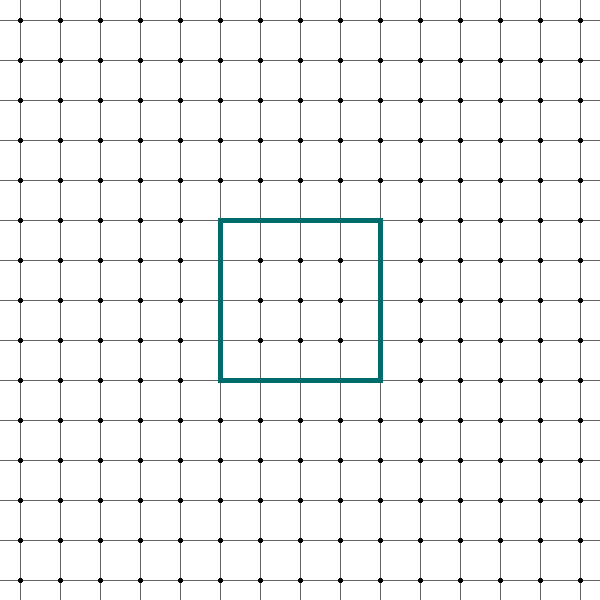
\includegraphics[width=\textwidth]{grid.png}
   \end{subfigure}
   \begin{subfigure}[c]{.1\textwidth}
    \centering
    \begin{tikzpicture}
     \draw[ultra thick,gevored,->] (0,0) -- (2,0);
    \end{tikzpicture}
   \end{subfigure}
   \begin{subfigure}[c]{.2\textwidth}
    \centering
    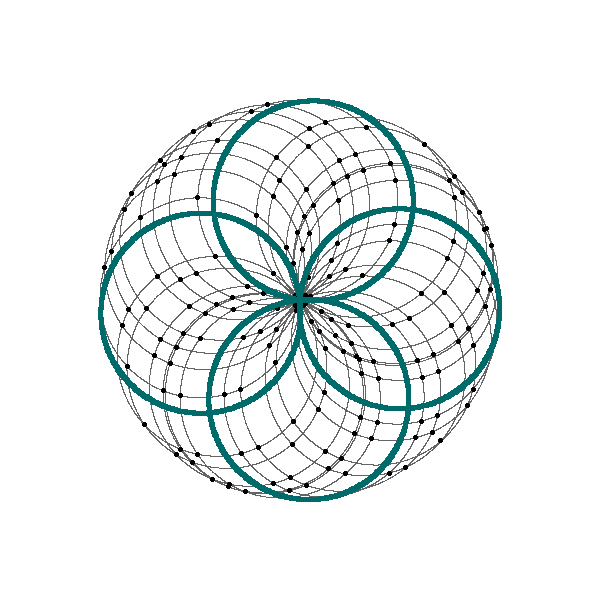
\includegraphics[width=\textwidth]{transformed_grid_1.png}
   \end{subfigure}
   \caption*{The transformation \alert{$(x,y) \mapsto (100(\sin x + \cos y),
   100(\cos x + \sin y))$}.}
  \end{figure}
 \end{block}

 \begin{exampleblock}{Rotations \& Reflections}
  We shall be interested in two specific plane transformations --
  \bfalert{rotations} and \bfalert{reflections}.

  \bfalert{Rotations} are plane transformations that, well ..., rotates the
  entire plane around a fixed point called \bfalert{anchor}. Applied to
  polygons, rotations may look like this:
  \begin{figure}[H]
   \centering
   \begin{subfigure}[t]{.25\textwidth}
    \centering
    \begin{tikzpicture}
     \foreach \angle/\name in {-54/A,18/B,90/C,162/D,234/E} {
      \tkzDefPoint(\angle:1){\name}
     }
     \tkzDrawPolygon[thick](A,B,C,D,E)
     \tkzDrawPoints(A,D,C,E)
     \tkzDefPointsBy[rotation=center B angle 60](A,B,C,D,E){A',B',C',D',E'}
     \tkzDrawPolygon[thick,color=gevodarkblue](A',B',C',D',E')
     \tkzDrawPoints[color=gevodarkblue](A',C',D',E')
     \tkzDrawPoint[color=gevored](B)
     \tkzMarkAngle[thick,color=gevored,size=1](C,B,C')
    \tkzLabelAngle[pos=0.5,color=gevored,xshift=-1mm](C,B,C'){\tiny
    $60^{\circ}$}
    \end{tikzpicture}
   \end{subfigure}
  \begin{subfigure}[t]{.25\textwidth}
   \centering
   \begin{tikzpicture}[scale=1.3,every node/.style={scale=1.3}]
    \foreach \angle/\name in {-54/A,18/B,90/C,162/D,234/E} {
     \tkzDefPoint(\angle:1){\name}
    }
    \tkzDefPoint(0,0){O}
    \tkzDrawPolygon[thick](A,B,C,D,E)
    \tkzDrawPoints(A,B,D,C,E)
    \tkzDrawPoint[color=gevored](O)
    \tkzDefPointsBy[rotation=center O angle -45](A,B,C,D,E){A',B',C',D',E'}
    \tkzDrawSegments[thick,color=gevored](O,C O,C')
    \tkzDrawPoint(C)
    \tkzDrawPolygon[thick,color=gevodarkblue](A',B',C',D',E')
    \tkzDrawPoints[color=gevodarkblue](A',B',C',D',E')
    \tkzMarkAngle[thick,color=gevored,size=0.7](C',O,C)
    \tkzLabelAngle[color=gevored,pos=0.5,xshift=0.5mm](C',O,C){\tiny
    $45^{ \circ }$}
   \end{tikzpicture}
  \end{subfigure}
   \caption*{Examples of \textcolor{gevodarkblue}{rotations} around a given
   \textcolor{gevored}{anchor}.}
  \end{figure}

  \bfalert{Reflections} are basically `mirrors'. They mirror each point in the
  plane through a given line called \bfalert{axis} (of reflection).
  \begin{figure}[H]
   \centering
   \begin{subfigure}[t]{.25\textwidth}
    \centering
    \begin{tikzpicture}
     \foreach \angle/\name in {-54/A,18/B,90/C,162/D,234/E} {
      \tkzDefPoint(\angle:1){\name}
     }
     \tkzDrawPolygon[thick](A,B,C,D,E)
     \tkzDrawPoints(A,B,C,D,E)
     \tkzDefPoints{0.7/1/O,0.7/-1/P}
     \tkzDrawLine[thick,color=gevored](O,P)
     \tkzDefPointsBy[reflection=over O--P](A,B,C,D,E){A',B',C',D',E'}
     \tkzDrawPolygon[thick,color=gevodarkblue](A',B',C',D',E')
     \tkzDrawPoints[color=gevodarkblue](A',B',C',D',E')
    \end{tikzpicture}
   \end{subfigure}
   \begin{subfigure}[t]{.25\textwidth}
    \centering
    \begin{tikzpicture}
     \clip (-1.1,-1.1) rectangle (1.1,1.5);
     \foreach \angle/\name in {-54/A,18/B,90/C,162/D,234/E} {
      \tkzDefPoint(\angle:1){\name}
     }
     \tkzDrawPolygon[thick](A,B,C,D,E)
     \tkzDrawPoints(A,B,C,D,E)
     \tkzDefPoints{-1/1.75/O,0.5/-1/P}
     \tkzDrawLine[thick,color=gevored,add=-0.2 and 0.2](O,P)
     \tkzDefPointsBy[reflection=over O--P](A,B,C,D,E){A',B',C',D',E'}
     \tkzDrawPolygon[thick,color=gevodarkblue](A',B',C',D',E')
     \tkzDrawPoints[color=gevodarkblue](A',B',C',D',E')
    \end{tikzpicture}
   \end{subfigure}
   \caption*{Examples of \textcolor{gevodarkblue}{reflections} over a given
   \textcolor{gevored}{axis}.}
  \end{figure}
 \end{exampleblock}

 \begin{alertblock}{Symmetries of Regular Polygons}
  Some \textbf{rotations} and \textbf{reflections} get along nicely with
  \textbf{regular polygons}. By this, we mean that they \alert{keep them
  intact}. We call them the \bfalert{symmetries} of the polygon.

  Each regular $n$-gon has multiple symmetries:
  \begin{itemize}[leftmargin=4ex]
   \item[\textcolor{gevodarkblue}{(r)}] \textbf{rotation} by $k \cdot 360^{
    \circ } / n$ for any $k$ between $1$ and $n$.
   \item[\textcolor{gevodarkblue}{(s)}] \textbf{reflection}
    \begin{itemize}[label=\textbullet]
    \item over lines passing through centres of opposite sides or through
     opposite vertices if $n$ is \bfalert{even};
    \item over lines passing through a centre of a side and the opposite vertex
     if $n$ is \bfalert{odd}.
   \end{itemize}
  \end{itemize}
  Therefore, an $n$-gon has $n$ rotational and $n$ reflectional symmetries.
  \begin{figure}[H]
   \centering
   \begin{subfigure}[c]{.25\textwidth}
    \centering
    \begin{tikzpicture}
     \foreach \angle/\name in {-30/A,90/B,210/C} {
      \tkzDefPoint(\angle:1){\name}
     }
     \tkzDefPoint(0,0){O}
     \tkzDrawPolygon[thick](A,B,C)
     \tkzDrawPoints(A,B)
     \tkzDrawPoint[color=gevored](C)
     \tkzDrawArc[color=gevored,thick,<-,delta=-10](O,B)(C)
     \tkzLabelArc[gevored,xshift=-6mm](O,B,C){\footnotesize $120^{ \circ }$}
     \tkzDrawArc[color=gevored,thick,<-,delta=-10](O,A)(B)
     \tkzDrawArc[color=gevored,thick,<-,delta=-10](O,C)(A)
     \tkzLabelArc[gevored,yshift=-4mm,xshift=1mm](O,C,A){\footnotesize $360^{
     \circ }$}
     \tkzLabelArc[gevored,xshift=2.5cm,yshift=1.04cm](O,A,B){\footnotesize $240^{
     \circ }$}
    \end{tikzpicture}
   \end{subfigure}
   \begin{subfigure}[c]{.25\textwidth}
    \centering
    \begin{tikzpicture}
     \foreach \angle/\name in {-54/A,18/B,90/C,162/D,234/E} {
      \tkzDefPoint(\angle:1){\name}
     }
     \foreach \p/\q in {A/B,B/C,C/D,D/E,E/A} {
      \tkzDefMidPoint(\p,\q)
      \tkzGetPoint{S\p\q}
     }
     \tkzDefPoint(0,0){O}
     \tkzDrawPolygon[thick](A,B,C,D,E)
     \tkzDrawLine[thick,color=gevored,dashed](SEA,C)
     \tkzDrawLine[thick,color=gevored,dashed](SAB,D)
     \tkzDrawLine[thick,color=gevored,dashed](SBC,E)
     \tkzDrawLine[thick,color=gevored,dashed](SCD,A)
     \tkzDrawLine[thick,color=gevored,dashed](SDE,B)
     \tkzDrawPoints(A,B,C,D,E)
    \end{tikzpicture}
   \end{subfigure}

   \caption*{Examples of regular polygon \alert{symmetries}.}
  \end{figure}

  Moreover, symmetries (being functions) can be \bfalert{chained} or
  \bfalert{composed}, creating new symmetries. We'll label rotations by the
  letter $r$ and reflections by $s$. A \bfalert{chain} or \bfalert{composition}
  is read left-to-right, that is, $sr$ means `apply $s$ first, then $r$'.
  \begin{figure}[H]
   \centering
   \begin{tikzpicture}[every node/.style = {scale=1.2}]
    \foreach \an/\name in {0/a,60/b,120/c,180/d,240/e,300/f} {
     \tkzDefPoint(\an:1){\name}
    }
    \tkzDrawPolygon[thick](a,b,c,d,e,f)
    \tkzLabelPoint[right](a){$1$}
    \tkzLabelPoint[above right](b){$2$}
    \tkzLabelPoint[above left](c){$3$}
    \tkzLabelPoint[left](d){$4$}
    \tkzLabelPoint[below left](e){$5$}
    \tkzLabelPoint[below right](f){$6$}

    \tkzDrawLine[dashed,thick,gevored,add=.5 and .5](c,f)
    \tkzDrawPoints(a,b,c,d,e,f)

    \coordinate (h1) at ($(a) + (0.5,0.5)$);
    \coordinate (h2) at ($(h1) + (2,0)$);
    
    \draw[thick,gevored,-Latex,bend left=30] (h1) to
     node[midway,gevored,yshift=3mm] {$s$} (h2);

    \tkzDefPoint(6,0){a1}
    \tkzDefPointsBy[translation=from a to a1](b,c,d,e,f){b1,c1,d1,e1,f1}
    \tkzDrawPolygon[thick](a1,b1,c1,d1,e1,f1)
    \tkzLabelPoint[right](a1){$5$}
    \tkzLabelPoint[above right](b1){$4$}
    \tkzLabelPoint[above left](c1){$3$}
    \tkzLabelPoint[left](d1){$2$}
    \tkzLabelPoint[below left](e1){$1$}
    \tkzLabelPoint[below right](f1){$6$}
    \tkzDrawPoints(a1,b1,c1,d1,e1,f1)

    \tkzDefPoint(5,0){o}
    \tkzDrawPoint[fill=none,gevodarkblue,thick](o)
    \tkzDrawArc[R,thick,gevodarkblue,->](o,0.5)(0,120)

    \coordinate (g1) at ($(a1) + (0.5,0.5)$);
    \coordinate (g2) at ($(g1) + (2,0)$);

    \draw[thick,gevodarkblue,-Latex,bend left=30] (g1) to
     node[midway,gevodarkblue,yshift=3mm] {$r$} (g2);

    \tkzDefPoint(11,0){a2}
    \tkzDefPointsBy[translation=from a1 to a2](b1,c1,d1,e1,f1){b2,c2,d2,e2,f2}
    \tkzDrawPolygon[thick](a2,b2,c2,d2,e2,f2)
    \tkzLabelPoint[right](a2){$1$}
    \tkzLabelPoint[above right](b2){$6$}
    \tkzLabelPoint[above left](c2){$5$}
    \tkzLabelPoint[left](d2){$4$}
    \tkzLabelPoint[below left](e2){$3$}
    \tkzLabelPoint[below right](f2){$2$}
    \tkzDrawPoints(a2,b2,c2,d2,e2,f2)

    \tkzDrawLine[thick,dotted,add=.5 and .5,nottblue](a2,d2)
    \tkzLabelLine[pos=-0.3,nottblue,yshift=3mm](a2,d2){$?$}
    \tkzDrawPoints(a2,b2,c2,d2,e2,f2)
   \end{tikzpicture}
   \caption*{Example of the composition $\mathbf{sr}$ of a reflection
   $\textcolor{gevored}{s}$ and a rotation $\textcolor{gevodarkblue}{r}$.}
  \end{figure}

  \textbf{The order of composition matters!}
  \begin{figure}[H]
   \centering
   \begin{tikzpicture}[scale=0.9,every node/.style = {scale=0.9}]
    \begin{scope}
     \foreach \an/\name in {0/a,60/b,120/c,180/d,240/e,300/f} {
      \tkzDefPoint(\an:1){\name}
     }
     \tkzDrawPolygon[thick](a,b,c,d,e,f)
     \tkzLabelPoint[right](a){$1$}
     \tkzLabelPoint[above right](b){$2$}
     \tkzLabelPoint[above left](c){$3$}
     \tkzLabelPoint[left](d){$4$}
     \tkzLabelPoint[below left](e){$5$}
     \tkzLabelPoint[below right](f){$6$}

     \tkzDrawLine[dashed,thick,gevored,add=.5 and .5](b,e)
     \tkzDrawPoints(a,b,c,d,e,f)

     \coordinate (h1) at ($(a) + (0.5,0.5)$);
     \coordinate (h2) at ($(h1) + (1,0)$);
     
     \draw[thick,gevored,-Latex,bend left=30] (h1) to
      node[midway,gevored,yshift=3mm] {$s$} (h2);

     \tkzDefPoint(5,0){a1}
     \tkzDefPointsBy[translation=from a to a1](b,c,d,e,f){b1,c1,d1,e1,f1}
     \tkzDrawPolygon[thick](a1,b1,c1,d1,e1,f1)
     \tkzLabelPoint[right](a1){$3$}
     \tkzLabelPoint[above right](b1){$2$}
     \tkzLabelPoint[above left](c1){$1$}
     \tkzLabelPoint[left](d1){$6$}
     \tkzLabelPoint[below left](e1){$5$}
     \tkzLabelPoint[below right](f1){$4$}
     \tkzDrawPoints(a1,b1,c1,d1,e1,f1)

     \tkzDefPoint(4,0){o}
     \tkzDrawPoint[fill=none,gevodarkblue,thick](o)
     \tkzDrawArc[R,thick,gevodarkblue,->](o,0.5)(0,240)

     \coordinate (g1) at ($(a1) + (0.5,0.5)$);
     \coordinate (g2) at ($(g1) + (1,0)$);

     \draw[thick,gevodarkblue,-Latex,bend left=30] (g1) to
      node[midway,gevodarkblue,yshift=3mm] {$r$} (g2);

     \tkzDefPoint(9,0){a2}
     \tkzDefPointsBy[translation=from a1 to a2](b1,c1,d1,e1,f1){b2,c2,d2,e2,f2}
     \tkzDrawPolygon[thick](a2,b2,c2,d2,e2,f2)
     \tkzLabelPoint[right](a2){$1$}
     \tkzLabelPoint[above right](b2){$6$}
     \tkzLabelPoint[above left](c2){$5$}
     \tkzLabelPoint[left](d2){$4$}
     \tkzLabelPoint[below left](e2){$3$}
     \tkzLabelPoint[below right](f2){$2$}
     \tkzDrawPoints(a2,b2,c2,d2,e2,f2)
     
     \tkzDrawLine[ultra thick,dotted,add=.5 and .5,nottblue](a2,d2)
     \tkzDrawPoints(a2,b2,c2,d2,e2,f2)
    \end{scope}
    \begin{scope}[xshift=11.3cm]
     \node at (0,0) {\huge $ \neq $};
    \end{scope}
    \begin{scope}[xshift=14cm]
     \foreach \an/\name in {0/a,60/b,120/c,180/d,240/e,300/f} {
      \tkzDefPoint(\an:1){\name}
     }
     \tkzDrawPolygon[thick](a,b,c,d,e,f)
     \tkzLabelPoint[right](a){$1$}
     \tkzLabelPoint[above right](b){$2$}
     \tkzLabelPoint[above left](c){$3$}
     \tkzLabelPoint[left](d){$4$}
     \tkzLabelPoint[below left](e){$5$}
     \tkzLabelPoint[below right](f){$6$}

     \tkzDefPoint(0,0){o}
     \tkzDrawPoint[fill=none,gevodarkblue,thick](o)
     \tkzDrawArc[R,thick,gevodarkblue,->](o,0.5)(0,240)

     \tkzDrawPoints(a,b,c,d,e,f)

     \coordinate (h1) at ($(a) + (0.5,0.5)$);
     \coordinate (h2) at ($(h1) + (1,0)$);
     
     \draw[thick,gevodarkblue,-Latex,bend left=30] (h1) to
      node[midway,gevodarkblue,yshift=3mm] {$r$} (h2);

     \tkzDefPoint(5,0){a1}
     \tkzDefPointsBy[translation=from a to a1](b,c,d,e,f){b1,c1,d1,e1,f1}
     \tkzDrawPolygon[thick](a1,b1,c1,d1,e1,f1)
     \tkzLabelPoint[right](a1){$3$}
     \tkzLabelPoint[above right](b1){$4$}
     \tkzLabelPoint[above left](c1){$5$}
     \tkzLabelPoint[left](d1){$6$}
     \tkzLabelPoint[below left](e1){$1$}
     \tkzLabelPoint[below right](f1){$2$}
     \tkzDrawPoints(a1,b1,c1,d1,e1,f1)

     \tkzDrawLine[dashed,thick,gevored,add=.5 and .5](b1,e1)

     \coordinate (g1) at ($(a1) + (0.5,0.5)$);
     \coordinate (g2) at ($(g1) + (1,0)$);

     \draw[thick,gevored,-Latex,bend left=30] (g1) to
      node[midway,gevored,yshift=3mm] {$s$} (g2);

     \tkzDefPoint(9,0){a2}
     \tkzDefPointsBy[translation=from a1 to a2](b1,c1,d1,e1,f1){b2,c2,d2,e2,f2}
     \tkzDrawPolygon[thick](a2,b2,c2,d2,e2,f2)
     \tkzLabelPoint[right](a2){$5$}
     \tkzLabelPoint[above right](b2){$4$}
     \tkzLabelPoint[above left](c2){$3$}
     \tkzLabelPoint[left](d2){$2$}
     \tkzLabelPoint[below left](e2){$1$}
     \tkzLabelPoint[below right](f2){$6$}
     \tkzDrawPoints(a2,b2,c2,d2,e2,f2)
     
     \tkzDrawLine[ultra thick,dotted,add=.5 and .5,nottblue](c2,f2)
     \tkzDrawPoints(a2,b2,c2,d2,e2,f2)
    \end{scope}
   \end{tikzpicture}
  \end{figure}
  In general, a composition of
  \begin{itemize}[label=\textcolor{gevodarkblue}{\textbullet},leftmargin=3ex]
   \item a \textbf{rotation} and a \textbf{rotation} is again a
    \textbf{rotation},
   \item a \textbf{rotation} and a \textbf{reflection} (in any order) is a
    \textbf{reflection},
   \item a \textbf{reflection} and a \textbf{reflection} is a \textbf{rotation}.
  \end{itemize}
 \end{alertblock}

\end{column}
\separatorcolumn

\begin{column}{\colwidth}

 \begin{block}{Generating Symmetries}
  \textbf{Question}: If I can compose symmetries, how many (and which)
  symmetries are enough to generate (create by composition) all the others?

  \textbf{Answer}: Just two are enough. Basically, I need to be able to generate
  the smallest rotation (that is, rotation by $360^{ \circ } / n$) and any
  reflection. Composing these two gives me all the other rotations and
  reflections.

  Let's see this on a regular pentagon. Here, $\textcolor{gevodarkblue}{r}$
  denotes the rotation by $360^{ \circ } / 5 = 72^{ \circ }$ and
  $\textcolor{gevored}{s}$ denotes the `vertical' reflection.
  \begin{figure}[H]
   \centering
   \begin{subfigure}[b]{.3\textwidth}
    \centering
    \begin{tikzpicture}
     \foreach \n/\name in {1/a,2/b,3/c,4/d,5/e} {
      \pgfmathsetmacro{\an}{(\n - 1) * 72 + 18}
      \tkzDefPoint(\an:1){\name}
     }
     \tkzDrawPolygon[thick](a,b,c,d,e)

     \tkzDefPoint(0,0){o}
     \tkzDrawPoint[fill=none,gevodarkblue,thick](o)
     \tkzDrawArc[R,thick,gevodarkblue,arrows={->[width=10pt,length=8pt]}](o,0.5)(18,90)

     \tkzDrawPoints(a,b,c,d,e)

    \end{tikzpicture}
    \caption*{Rotation by $72^{ \circ }$, denoted
    $\textcolor{gevodarkblue}{r}$.}
   \end{subfigure}
   \begin{subfigure}[b]{.3\textwidth}
    \centering
    \begin{tikzpicture}
     \foreach \n/\name in {1/a,2/b,3/c,4/d,5/e} {
      \pgfmathsetmacro{\an}{(\n - 1) * 72 + 18}
      \tkzDefPoint(\an:1){\name}
     }
     \tkzDrawPolygon[thick](a,b,c,d,e)

     \tkzDefPoint(0,0){o}
     \tkzDrawPoint[fill=none,gevodarkblue,thick](o)
     \tkzDrawArc[R,thick,gevodarkblue,arrows={->[width=10pt,length=8pt]}](o,0.5)(18,162)

     \tkzDrawPoints(a,b,c,d,e)

    \end{tikzpicture}
    \caption*{The composition $\textcolor{gevodarkblue}{rr} =
    \textcolor{gevodarkblue}{r^2}$.}
   \end{subfigure}
   \begin{subfigure}[b]{.3\textwidth}
    \centering
    \begin{tikzpicture}
     \foreach \n/\name in {1/a,2/b,3/c,4/d,5/e} {
      \pgfmathsetmacro{\an}{(\n - 1) * 72 + 18}
      \tkzDefPoint(\an:1){\name}
     }
     \tkzDrawPolygon[thick](a,b,c,d,e)

     \tkzDefPoint(0,0){o}
     \tkzDrawPoint[fill=none,gevodarkblue,thick](o)
     \tkzDrawArc[R,thick,gevodarkblue,arrows={->[width=10pt,length=8pt]}](o,0.5)(18,234)

     \tkzDrawPoints(a,b,c,d,e)

    \end{tikzpicture}
    \caption*{The composition $\textcolor{gevodarkblue}{r^3}$.}
   \end{subfigure}
   \begin{subfigure}[b]{.3\textwidth}
    \centering
    \begin{tikzpicture}
     \foreach \n/\name in {1/a,2/b,3/c,4/d,5/e} {
      \pgfmathsetmacro{\an}{(\n - 1) * 72 + 18}
      \tkzDefPoint(\an:1){\name}
     }
     \tkzDrawPolygon[thick](a,b,c,d,e)

     \tkzDefPoint(0,0){o}
     \tkzDrawPoint[fill=none,gevodarkblue,thick](o)
     \tkzDrawArc[R,thick,gevodarkblue,arrows={->[width=10pt,length=8pt]}](o,0.5)(18,306)

     \tkzDrawPoints(a,b,c,d,e)

    \end{tikzpicture}
    \caption*{The composition $\textcolor{gevodarkblue}{r^4}$.}
   \end{subfigure}
   \begin{subfigure}[b]{.3\textwidth}
    \centering
    \begin{tikzpicture}
     \foreach \n/\name in {1/a,2/b,3/c,4/d,5/e} {
      \pgfmathsetmacro{\an}{(\n - 1) * 72 + 18}
      \tkzDefPoint(\an:1){\name}
     }
     \tkzDrawPolygon[thick](a,b,c,d,e)

     \tkzDefPoint(0,0){o}
     \tkzDrawPoint[fill=none,gevodarkblue,thick](o)
     \tkzDrawArc[R,thick,gevodarkblue,arrows={->[width=10pt,length=8pt]}](o,0.5)(18,378)

     \tkzDrawPoints(a,b,c,d,e)

    \end{tikzpicture}
    \caption*{The composition $\textcolor{gevodarkblue}{r^5}$.}
   \end{subfigure}
   \begin{subfigure}[b]{.3\textwidth}
    \centering
    \begin{tikzpicture}
     \foreach \n/\name in {1/a,2/b,3/c,4/d,5/e} {
      \pgfmathsetmacro{\an}{(\n - 1) * 72 + 18}
      \tkzDefPoint(\an:1){\name}
     }
     \tkzDrawPolygon[thick](a,b,c,d,e)


     \tkzDefMidPoint(d,e)\tkzGetPoint{m}
     \tkzDrawLine[dashed,thick,gevored,add=.25 and .25](b,m)
     \tkzDrawPoints(a,b,c,d,e)

    \end{tikzpicture}
    \caption*{`Vertical' reflection, denoted $\textcolor{gevored}{s}$.}
   \end{subfigure}
   \begin{subfigure}[b]{.3\textwidth}
    \centering
    \begin{tikzpicture}
     \foreach \n/\name in {1/a,2/b,3/c,4/d,5/e} {
      \pgfmathsetmacro{\an}{(\n - 1) * 72 + 18}
      \tkzDefPoint(\an:1){\name}
     }
     \tkzDrawPolygon[thick](a,b,c,d,e)


     \tkzDefMidPoint(a,b)\tkzGetPoint{m}
     \tkzDrawLine[dashed,thick,gevored,add=.25 and .25](d,m)
     \tkzDrawPoints(a,b,c,d,e)

    \end{tikzpicture}
    \caption*{The composition
    $\textcolor{gevodarkblue}{r}\textcolor{gevored}{s}$.}
   \end{subfigure}
   \begin{subfigure}[b]{.3\textwidth}
    \centering
    \begin{tikzpicture}
     \foreach \n/\name in {1/a,2/b,3/c,4/d,5/e} {
      \pgfmathsetmacro{\an}{(\n - 1) * 72 + 18}
      \tkzDefPoint(\an:1){\name}
     }
     \tkzDrawPolygon[thick](a,b,c,d,e)


     \tkzDefMidPoint(c,d)\tkzGetPoint{m}
     \tkzDrawLine[dashed,thick,gevored,add=.25 and .25](a,m)
     \tkzDrawPoints(a,b,c,d,e)

    \end{tikzpicture}
    \caption*{The composition
    $\textcolor{gevodarkblue}{r^2}\textcolor{gevored}{s}$.}
   \end{subfigure}
   \begin{subfigure}[b]{.3\textwidth}
    \centering
    \begin{tikzpicture}
     \foreach \n/\name in {1/a,2/b,3/c,4/d,5/e} {
      \pgfmathsetmacro{\an}{(\n - 1) * 72 + 18}
      \tkzDefPoint(\an:1){\name}
     }
     \tkzDrawPolygon[thick](a,b,c,d,e)


     \tkzDefMidPoint(a,e)\tkzGetPoint{m}
     \tkzDrawLine[dashed,thick,gevored,add=.25 and .25](c,m)
     \tkzDrawPoints(a,b,c,d,e)

    \end{tikzpicture}
    \caption*{The composition
    $\textcolor{gevodarkblue}{r^3}\textcolor{gevored}{s}$.}
   \end{subfigure}
   \begin{subfigure}[b]{.3\textwidth}
    \centering
    \begin{tikzpicture}
     \foreach \n/\name in {1/a,2/b,3/c,4/d,5/e} {
      \pgfmathsetmacro{\an}{(\n - 1) * 72 + 18}
      \tkzDefPoint(\an:1){\name}
     }
     \tkzDrawPolygon[thick](a,b,c,d,e)


     \tkzDefMidPoint(b,c)\tkzGetPoint{m}
     \tkzDrawLine[dashed,thick,gevored,add=.25 and .25](e,m)
     \tkzDrawPoints(a,b,c,d,e)

    \end{tikzpicture}
    \caption*{The composition
    $\textcolor{gevodarkblue}{r^4}\textcolor{gevored}{s}$.}
   \end{subfigure}
   \caption*{All symmetries of the regular pentagon written as compositions of
   $\textcolor{gevodarkblue}{r}$ and $\textcolor{gevored}{s}$.}
  \end{figure}

  \textbf{Question}: Given two symmetries, how do I know I can generate the rest
  using only these two?

  \textbf{Answer}: It of course depends on their type.
  \begin{itemize}[label=\textcolor{gevodarkblue}{\textbullet},leftmargin=3ex]
   \item If I'm given 2 rotations, I can never generate all symmetries because
    composing rotations doesn't yield a reflection.
   \item If I'm given a rotation and a reflection, then the rotation must be by
    $k \cdot 360^{ \circ } / n$ with $k$ \textbf{coprime to} $n$. Otherwise I can
    never generate the rotation by $360^{ \circ } / n$. The reflection can be of
    any kind.
   \item If I'm given two reflections, their composition must be a rotation by $k
    \cdot 360^{ \circ } / n$ with $k$ \textbf{coprime to} $n$ for the same reason
    as above.
  \end{itemize}
 \end{block}

 \begin{block}{Vocabulary}
   \begin{center}
   {\def\arraystretch{1.2}\tabcolsep=10pt
    \begin{tabular}{c | c | p{.5\textwidth}}
     \textbf{English} & \textbf{Czech} & \textbf{Definition}\\
     \toprule
     Segment & Úsečka & Straight finite line connecting two points.\\
     Polygon & Mnohoúhelník & Closed 2D shape made of segments.\\
     Vertex & Vrchol & Any of the endpoints of the segments forming a polygon.\\
     Edge & Hrana & Any of the segments forming a polygon.\\
     Triangle & Trojúhelník & A polygon with 3 vertices.\\
     Quadrilateral & Čtyřúhelník & A polygon with 4 vertices.\\
     Internal/External angle & Vnitřní/Vnější úhel & The angle on the
     inside/outside of a polygon formed by its edges.\\
     Convex & Konvexní & A polygon whose internal angles don't exceed 180$^{
     \circ }$.\\
     Equilateral & Rovnostranný & Describes a polygon with all sides of equal
     length.\\
     Trapezoid & Lichoběžník & A quadrilateral with a pair of parallel sides.\\
     Parallelogram & Rovnoběžník & A quadrilateral with two pairs of parallel
     sides.\\
     Rhombus & Kosočtverec & An equilateral parallelogram.\\
     Regular & Pravidelný & Describes an equilateral polygon with all angles of
     the same size.\\
     Square & Čtverec & A regular quadrilateral.
    \end{tabular}
   }
   \end{center}
 \end{block}

\end{column}
\separatorcolumn

\end{columns}
\end{frame}

\end{document}
